% ------------------------------------------------------------------------------
% TYPO3 Versie 10.0 - What's New (Dutch Version)
%
% @author	Michael Schams <schams.net>
% @license	Creative Commons BY-NC-SA 3.0
% @link		http://typo3.org/download/release-notes/whats-new/
% @language	Dutch
% ------------------------------------------------------------------------------

\section{Gebruikersinterface backend}
\begin{frame}[fragile]
	\frametitle{Gebruikersinterface backend}

	\begin{center}\huge{Hoofdstuk 1:}\end{center}
	\begin{center}\huge{\color{typo3darkgrey}\textbf{Gebruikersinterface backend}}\end{center}

\end{frame}

% ------------------------------------------------------------------------------
% Feature | 56213 | Allow sorting file list by file meta data title

\begin{frame}[fragile]
	\frametitle{Gebruikersinterface backend}
	\framesubtitle{Sortering bestandslijst}

	Bestanden kunnen gesorteerd wordt op de metadata-titel in het inhoudselement "Bestandskoppelingen".

	\begin{figure}
		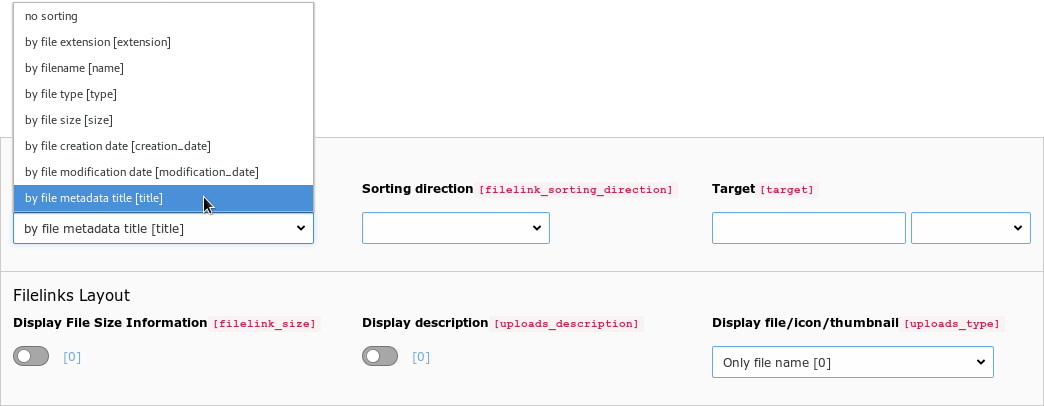
\includegraphics[width=0.90\linewidth]{BackendUserInterface/56213-FilelistSorting.png}
	\end{figure}

\end{frame}

% ------------------------------------------------------------------------------
% Feature | 85569 | Show scheduler information in the system information toolbar

\begin{frame}[fragile]
	\frametitle{Gebruikersinterface backend}
	\framesubtitle{Knoppenbalk systeeminformatie}

	De knoppenbalk systeeminformatie toont nu informatie over de TYPO3 taakplanner.

	\begin{figure}
		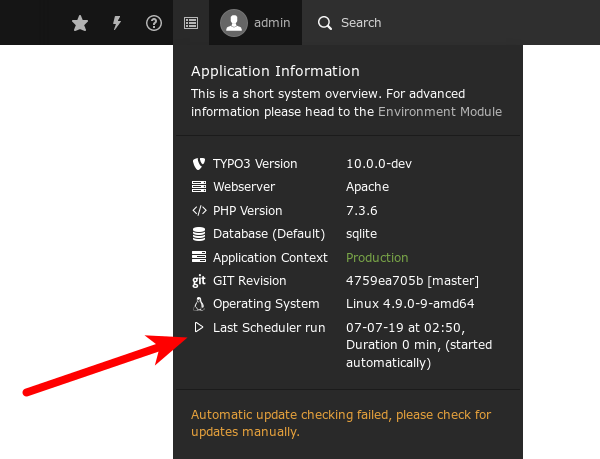
\includegraphics[width=0.50\linewidth]{BackendUserInterface/85569-SchedulerInfoInStatusBar.png}
	\end{figure}

\end{frame}

% ------------------------------------------------------------------------------
% Feature | 86629 | Implement LinkHandler for telephone numbers

\begin{frame}[fragile]
	\frametitle{Gebruikersinterface backend}
	\framesubtitle{Linkhandler}

	Een nieuwe linkhandler is toegevoegd waarmee redacteuren links kunnen maken naar
	telefoonnummers met het \texttt{tel:} protocol.

	\begin{figure}
		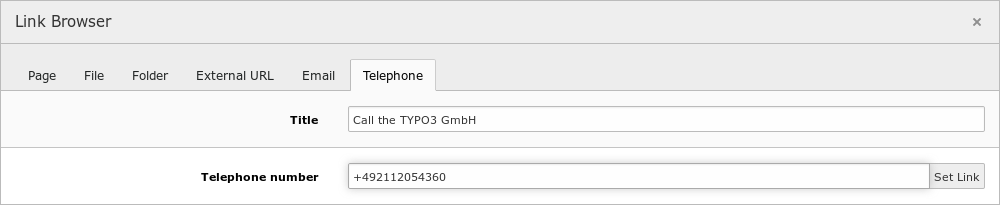
\includegraphics[width=0.90\linewidth]{BackendUserInterface/86629-TelephoneNumberLinkHandler.png}
	\end{figure}

	\begin{figure}
		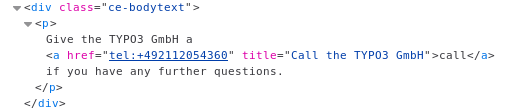
\includegraphics[width=0.60\linewidth]{BackendUserInterface/86629-TelephoneNumberLinkHandler2.png}
	\end{figure}

\end{frame}

% ------------------------------------------------------------------------------
% Feature | 87433 | Add changefreq and priority

\begin{frame}[fragile]
	\frametitle{Gebruikersinterface backend}
	\framesubtitle{SEO Sitemap (1)}

	\texttt{EXT:seo} ondersteunt nu wijzigingsfrequentie ne prioriteiten voor de sitemap.
	Pagina-eigenschappen (tab "SEO") bevat twee nieuwe velden.

	\begin{figure}
		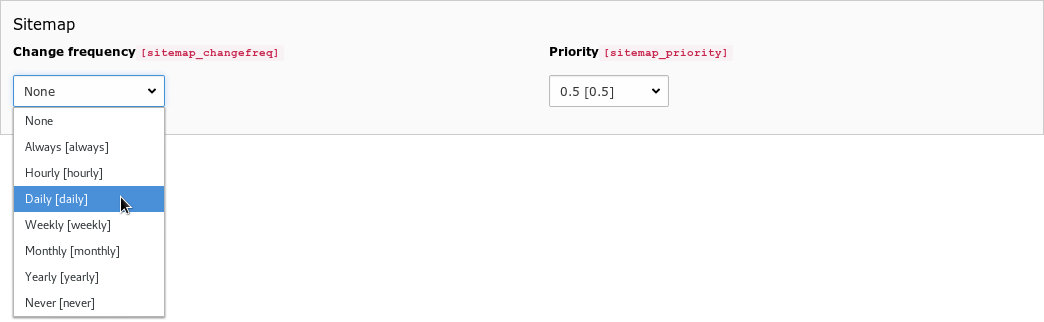
\includegraphics[width=0.90\linewidth]{BackendUserInterface/87433-SeoAddChangefreqAndPriority.png}
	\end{figure}

\end{frame}

% ------------------------------------------------------------------------------
% Feature | 87433 | Add changefreq and priority

\begin{frame}[fragile]
	\frametitle{Gebruikersinterface backend}
	\framesubtitle{SEO Sitemap (2)}

	% decrease font size for code listing
	\lstset{basicstyle=\tiny\ttfamily}

    Deze instellingen kunnen ook TypoScript gemaakt worden en worden overgezet naar velden
    in de database.

	\begin{lstlisting}
plugin.tx_seo {
  config {
    xmlSitemap {
      sitemaps {
        <unieke waarde> {
          provider = TYPO3\CMS\Seo\XmlSitemap\RecordsXmlSitemapDataProvider
          config {
            ...
            changeFreqField = news_changefreq
            priorityField = news_priority
            ...
          }
        }
      }
    }
  }
}
	\end{lstlisting}

\end{frame}

% ------------------------------------------------------------------------------
% Feature | 84757 | Double click in structure tree changes label

\begin{frame}[fragile]
	\frametitle{Changes for Integrators}
	\framesubtitle{Formulieren}

	% decrease font size for code listing
	\lstset{basicstyle=\tiny\ttfamily}

	Labels van formulierelementen kunnen bewerkt worden door te dubbelklikken op de titel in de boom.

	\begin{figure}
		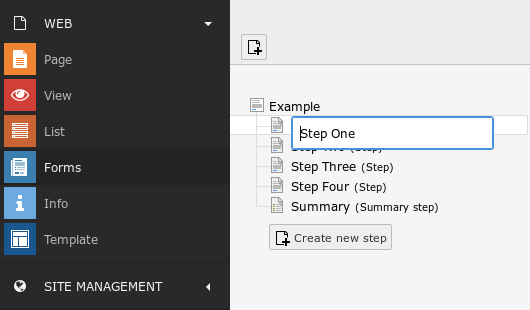
\includegraphics[width=0.60\linewidth]{ChangesForIntegrators/84757-DoubleClickToChangeLabel.png}
	\end{figure}

\end{frame}

% ------------------------------------------------------------------------------
